\documentclass[11pt]{article}
\usepackage[margin=1in]{geometry}
\usepackage{amsmath}
\usepackage{booktabs}
\usepackage{array}
\usepackage{graphicx}
\usepackage{float}
\usepackage[hidelinks]{hyperref}

\newcommand{\AtlasPending}[1]{\textbf{[PENDING: #1]}}

\title{Frequency-Coverage Limits in Assessing Gravity Signals from Oceanic Mass Redistribution}
\author{\AtlasPending{author list and affiliations}}
\date{Reproducible results draft; author metadata pending}

\begin{document}
\maketitle

\begin{abstract}
Oceanic mass redistribution produces direct gravitational attraction and, for
surface loads, elastic/potential and height responses over timescales from
seconds to months. We develop an evidence-bounded process--distance--instrument
framework with explicit source geometry, observation duration, spectral
coverage, and instrument-specific noise. The primary six-process production
ensemble contains 1,446 records of direct radial gravity; elastic and height
components are retained separately where evaluated and are not implied for
every process branch. None passes a predeclared 90\% signal-energy
coverage gate for the three admitted vertical-gravity literature anchors: tide,
storm surge, eddy and internal-wave signals have no overlapping band, whereas
tsunami and landslide records have only partial coverage. We therefore withhold
SNR classifications rather than extrapolating instrument curves. An independent
open-data Helgoland calculation reproduces the published BSH gravity-to-height
ratio within 15.6\%. The framework identifies frequency coverage, source geometry
and mass compensation as separate limits on defensible ocean-gravity
detectability statements.
\end{abstract}

\section{Introduction}
Environmental Newtonian-noise studies already quantify atmospheric, seismic,
and ocean-related gravitational disturbances for gravitational-wave facilities;
they are not instrument-noise calculations developed here. Likewise, terrestrial
gravimetry has detected non-tidal ocean loading during storm surges. The present
increment is a cross-process, cross-distance, cross-instrument assessment under
one auditable convention. It first asks whether available instrument evidence
covers enough signal energy to authorize a detectability decision. It does not
claim that the
underlying gravity kernels, loading theory, or individual instrument concepts
are new.

\section{Methods}
\subsection{Observables and sign conventions}
All kernels use SI units. For a surface mass anomaly $\Delta\sigma$,
\begin{equation}
 \Delta\mathbf{g}_{\mathrm{direct}}(\mathbf{r},t)
 =G\int_A \Delta\sigma(\mathbf{x},t)
 \frac{\mathbf{x}-\mathbf{r}}{|\mathbf{x}-\mathbf{r}|^3}\,\mathrm{d}A.
\end{equation}
For a volume-density anomaly $\rho'$, the analogous integral is evaluated over
volume. The gravity-gradient convention is
$T_{ij}=\partial g_i/\partial x_{\mathrm{observation},j}$. Direct attraction,
combined elastic gravity and vertical displacement are stored separately. The
LoadDef CE gravity term combines deformation and potential response according
to its source convention and is never represented as direct attraction.

\subsection{Earth, grid and coastal geometry}
Reference calculations include local planar, mean-radius spherical, and WGS~84
ellipsoidal geometry. Spherical and ellipsoidal cell areas are integrated in
their native surface coordinates. Missing ocean values, hard masks, and partial
coastal-cell fractions are explicit. Grid refinement and domain truncation are
tested before a dataset is admitted to a result.

For idealized compact surface anomalies evaluated against terrestrial
instruments, source cells and the station lie on a spherical Earth. Distance is
the great-circle surface standoff from the represented three-standard-deviation
source support. Compact anomalies translate parallel to an idealized coastline,
preventing a source cell from coinciding with the station. A rejected local-plane
near-field calculation is retained in the experiment preregistration history:
its midpoint quadrature exceeded the continuous-sheet amplitude bound and did
not enter the registered output.

\subsection{Ocean-process models}
The six process families are summarized in Table~\ref{tab:processes}. Surface
and compensated three-dimensional variants are retained only where physically
supported. Engineering fixtures used for software validation are excluded from
scientific uncertainty statements. Parameter values are linked to named events,
catalogue means or published ranges. They define sensitivity designs, not
occurrence probabilities or population percentiles. The mesoscale-eddy Gaussian
branch uses catalogue-scale amplitude, radius and propagation speed from
Chelton et al.~\cite{Chelton2011}. Surface-wave packets and density dipoles are
mass balanced before gravity integration.

\begin{table}[ht]
\centering
\caption{Primary direct-gravity representations in P1-E006. Record counts include repeated distances, durations or paired sensitivity points and are not counts of independent natural events.}
\label{tab:processes}
\begin{tabular}{>{\raggedright\arraybackslash}p{0.14\linewidth}>{\raggedright\arraybackslash}p{0.31\linewidth}>{\raggedright\arraybackslash}p{0.23\linewidth}r}
\toprule
Process & Evidence/representation & Independent physical family & Records \\
\midrule
Tide & 1-m M2 spherical-disk transfer & one geometry diagnostic; 5 distances $\times$ 32 durations & 160 \\
Storm surge & gridded 2022 Helgoland BSH field & one named model case & 1 \\
Eddy & catalogue-mean translating Gaussian SSH & one representative mean case; 5 distances & 5 \\
Internal wave & compensated density dipole & one model family; 128 paired sensitivities $\times$ 5 distances & 640 \\
Tsunami & mass-balanced Gaussian packet & one packet family; 96 paired sensitivities $\times$ 5 distances & 480 \\
Landslide & Storegga conserved relocation & one named extreme family; 32 paired sensitivities $\times$ 5 distances & 160 \\
\bottomrule
\end{tabular}
\end{table}

\subsection{Spectra and detectability}
For transient signals, expected matched-filter signal-to-noise ratio is
\begin{equation}
 \rho^2=4\int_{f_{\min}}^{f_{\max}}
 \frac{|\tilde{s}(f)|^2}{S_n(f)}\,\mathrm{d}f.
\end{equation}
Fourier normalization, detrending, one-sided PSD, and observation duration are
versioned. A classification is forbidden unless the instrument curve covers at
least 90\% of signal spectral energy. Vertical gravity, gravity gradient, and
gravitational-wave equivalent strain remain different observables and are never
merged into one sensitivity curve. The admitted vertical-gravity entries are an
iGrav quiet self-noise anchor and short-term AQG-A01 and FG5\#228 anchors; their
declared frequency intervals are not extrapolated.

\subsection{Parameter design and uncertainty}
Latin-hypercube and stratified designs are labelled as scenario envelopes unless
every dimension has a source-supported probability distribution. Engineering
ranges cannot be reported as probabilistic 5--95\% intervals. Density-compensated
models retain cancellation and far-field suppression rather than replacing them
with equivalent uncompensated water columns. Source standoffs are 10, 30, 100,
300 and 1,000~km, and every coverage-limited outcome is retained.

\section{Validation}
Analytic tests cover point masses, finite disks, rectangles, Gaussian sheets,
volume cells, gradient symmetry and trace, WGS~84 area, mass conservation, grid
convergence, domain truncation, and time/frequency normalization. The complete
software audit contains 461 passing tests and 12 passing subtests after the
structural-closure implementation.

The LoadDef v1.2.2 PREM/CE provider reproduces all 50 published benchmark rows
used by the project for angular distance, radial displacement and combined
elastic gravity~\cite{Martens2019}. Direct attraction is calculated independently;
LoadDef's Newtonian term is not added a second time.

The Helgoland model-only reproduction uses 242 BSH-HBMnoku files and 720 hourly
fields conservatively remapped to a 1/8-degree WGS~84 grid. Direct attraction,
combined elastic gravity and vertical displacement remain separate. After the
registered sign conversion at the literature-comparison boundary, the computed
gravity-to-height ratio is $-2.266$~nm~s$^{-2}$~mm$^{-1}$, compared with
$-2.684$~nm~s$^{-2}$~mm$^{-1}$ reported by Voigt et
al.~\cite{Voigt2024}. The 15.6\% difference passes the predeclared 20\% tolerance
for replacing SPOTL/Gutenberg--Bullen and a three-year tidal analysis with
LoadDef PREM/CE and the registered 30-day harmonic fit.

\section{Results}
Figure~\ref{fig:frequency} compares process timescales with the admitted
instrument-curve support. M2 tide and the M2 internal-wave branch lie near
$2.24\times10^{-5}$~Hz. Storm-surge and eddy ranges are lower. The three admitted
vertical-gravity anchors begin at $10^{-3}$~Hz. Tsunami characteristic content
crosses that edge, while the Storegga transition lies mainly below it; neither
has 90\% of signal energy inside a complete admitted band.

\begin{figure}[H]
\centering
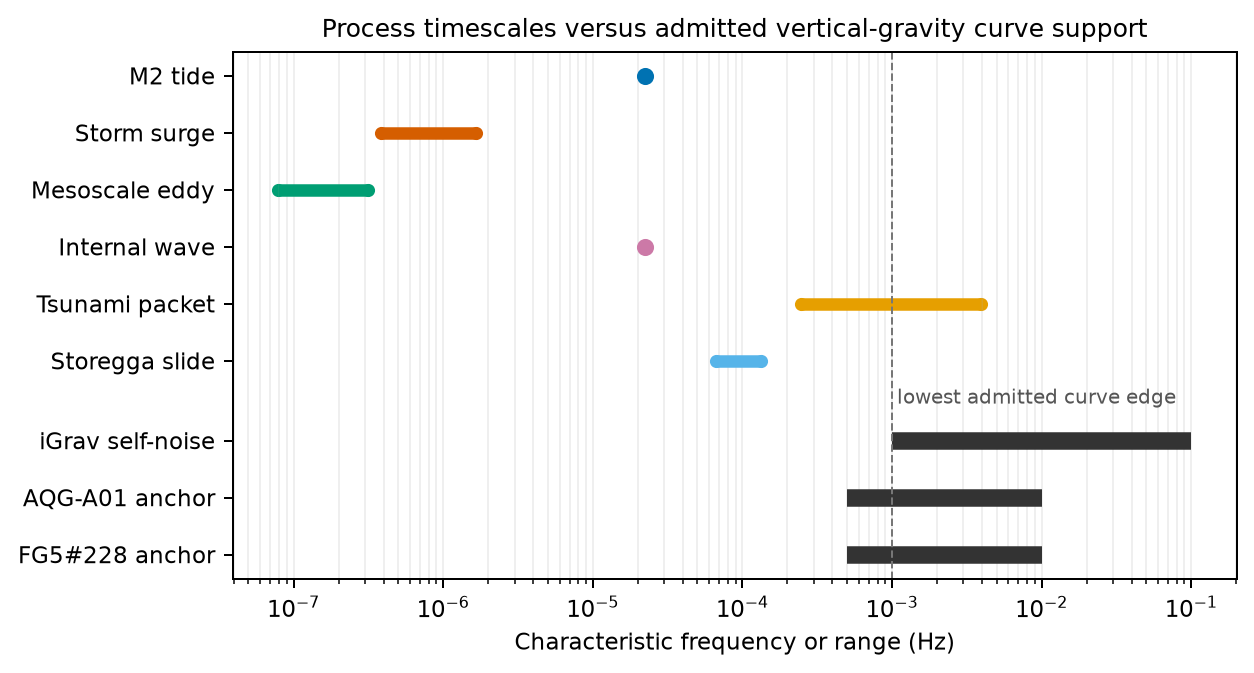
\includegraphics[width=0.96\linewidth]{../../reports/figures/paper1/p1_frequency_coverage.png}
\caption{Characteristic process frequencies and admitted vertical-gravity
curve support. Points denote fixed constituent frequencies and horizontal bars
denote sensitivity ranges. Curve limits are not extrapolated.}
\label{fig:frequency}
\end{figure}

The resulting coverage matrix is shown in Figure~\ref{fig:matrix}. All 806
long-period records have no covered spectral interval for any admitted curve.
All 640 tsunami and Storegga records have some overlapping bins but fail the
90\% energy criterion. Consequently no production record is labelled detectable
or undetectable. This differs from a statement of zero SNR: available curve
support is insufficient to make the comparison.

\begin{figure}[H]
\centering
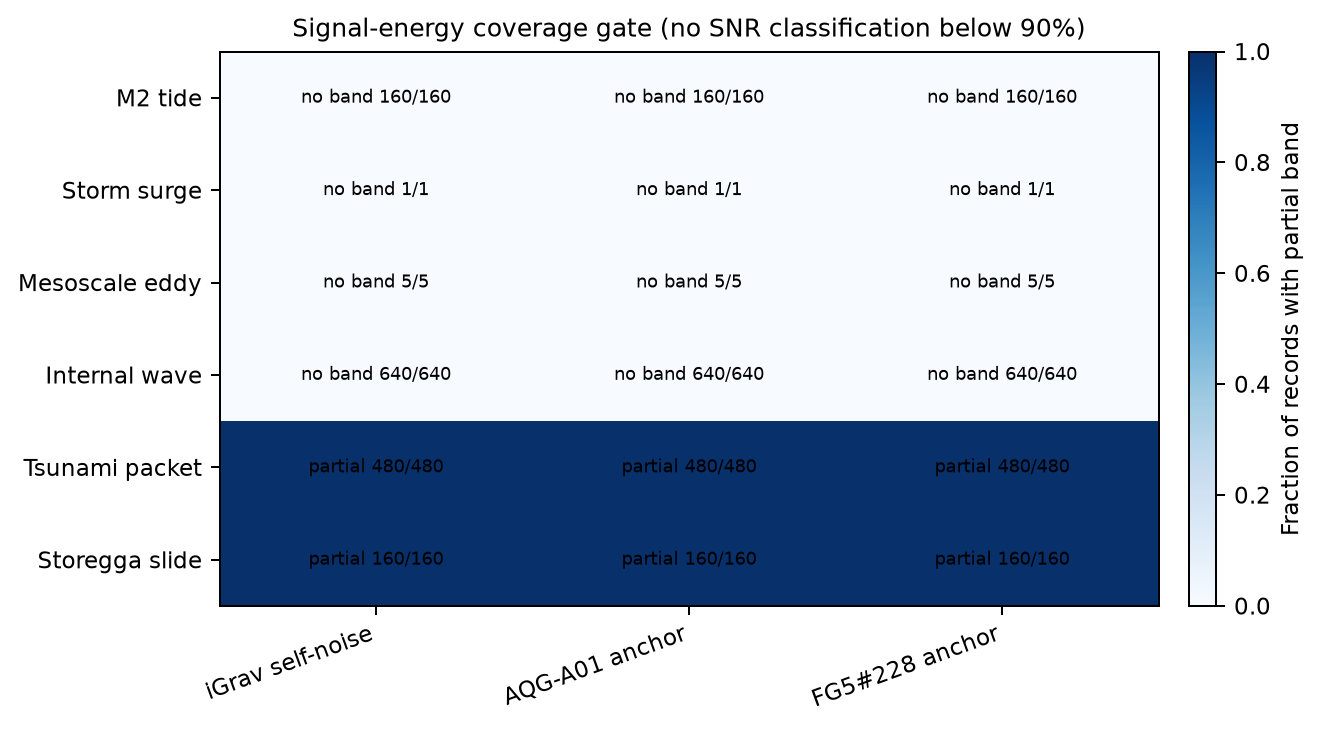
\includegraphics[width=0.94\linewidth]{../../reports/figures/paper1/p1_process_instrument_matrix.png}
\caption{Process--instrument signal-energy coverage. ``No band'' means fewer
than two positive-frequency bins overlap a curve; ``partial'' means overlap is
present but covers less than 90\% of signal energy.}
\label{fig:matrix}
\end{figure}

Direct radial-gravity amplitudes decay with spherical surface standoff
(Figure~\ref{fig:distance}). The Storegga named-event branch has the largest
primary-branch envelope, with median peak amplitude decreasing from about
$9.5\times10^{-9}$~m~s$^{-2}$ at 10~km to $1.0\times10^{-10}$~m~s$^{-2}$ at
1,000~km. The compensated tsunami envelope decreases from approximately
$3.1$--$6.5\times10^{-10}$ to $4.9$--$12.7\times10^{-12}$~m~s$^{-2}$ across the
same standoffs. The internal-wave dipole has an off-axis maximum near 100~km,
illustrating why amplitude need not decrease monotonically inside a compensated
source's near field.

\begin{figure}[H]
\centering
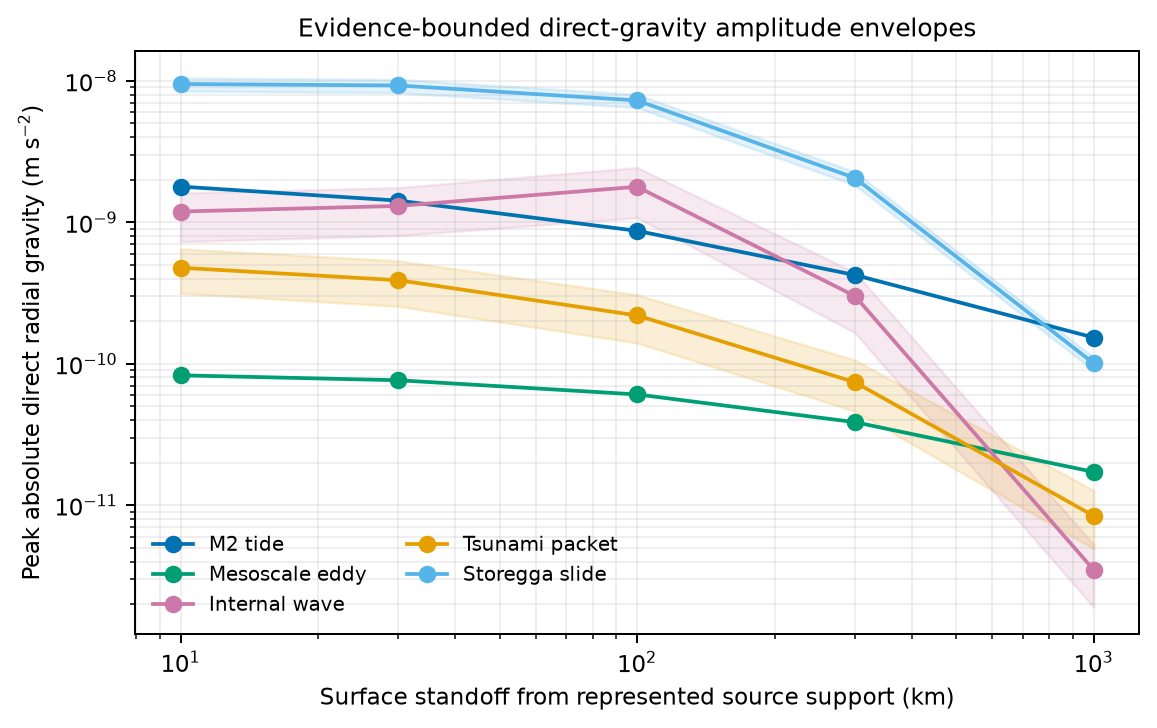
\includegraphics[width=0.96\linewidth]{../../reports/figures/paper1/p1_distance_amplitude_envelopes.png}
\caption{Peak absolute direct radial gravity versus surface standoff. Lines show
the median sensitivity design and shading spans the sampled minimum and maximum;
shading is not a probability interval.}
\label{fig:distance}
\end{figure}

Figure~\ref{fig:sensitivity} separates the density/displacement, wave-packet and
slide-parameter envelopes. Every tsunami crest and trough pair cancels signed
surface mass to numerical tolerance, and every slide record relocates rather
than creates solid mass.

\begin{figure}[H]
\centering
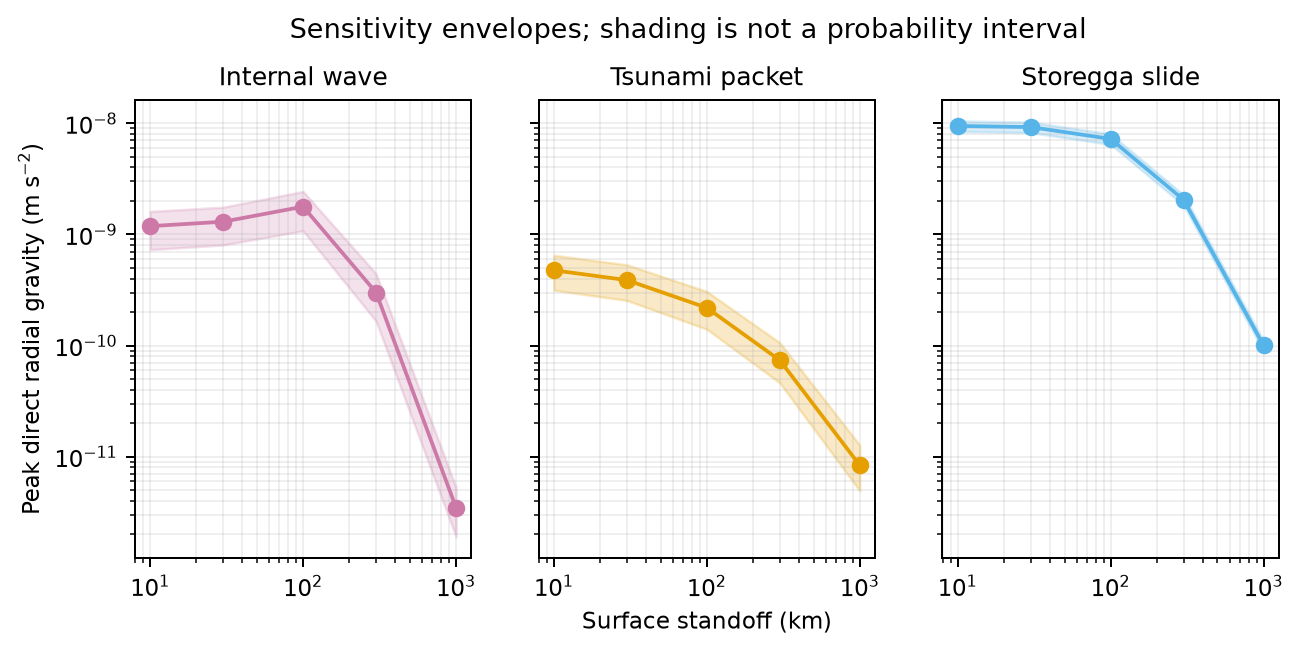
\includegraphics[width=0.98\linewidth]{../../reports/figures/paper1/p1_sensitivity_envelopes.png}
\caption{Evidence-bounded parameter sensitivity for three primary branches.
The bands represent design extrema and must not be read as confidence or
credible intervals.}
\label{fig:sensitivity}
\end{figure}

A separate registered structural-closure experiment maps the
$3.0\times10^{15}$~J Tohoku propagated-energy estimate (6\% uncertainty)
reported by Tang et al.~\cite{Tang2012} to the same idealized mass-balanced
Gaussian packet. Under the declared linear-long-wave convention
$E=\rho g\int\eta^2\,\mathrm{d}A$, the 300--400~km separation sensitivity gives
a central crest amplitude of 4.359~m and an energy-uncertainty range of
4.226--4.488~m. This branch is deliberately separate from the 1.0--1.8~m
deep-ocean amplitude-normalized branch; their difference measures
normalization/model-form sensitivity and is not combined as a probability
interval.

\section{Discussion}
The principal result is a boundary between classified, coverage-limited, and
physically suppressed signals. Compensated internal structures can decay much
faster than surface-load estimates, while long-period processes may be strong
but unclassifiable when empirical noise curves do not cover their frequency
band. An amplitude--noise intersection is not a sufficient detectability test:
observation duration and spectral energy coverage must be evaluated first.

The absence of a production SNR classification is therefore informative. It
identifies a data requirement---site and instrument noise curves extending into
the process band---rather than an invitation to extend short-term white-noise
anchors by assumption. Environmental Newtonian-noise calculations expressed as
gravitational-wave strain are likewise not interchangeable with gravimeter
self-noise~\cite{Brundu2022}.

The Helgoland reproduction supplies an independent positive validation of the
elastic loading scale but not of observation/model correlation. The reported
85~nm~s$^{-2}$ and $-34$~mm extrema are observations, not BSH model acceptance
targets. Reproducing the reported correlation and RMS reduction would require
authenticated iGrav047 data and a paper-equivalent processed 2022 GNSS series.

\section{Conclusions}
The current public instrument anchors do not support a decision-grade
cross-process detectability map: no production record reaches the required
signal-energy coverage. This result does not imply absent physical signals or
universal non-detectability. It establishes the frequency support that future
site-specific noise measurements must provide, while the direct-gravity
scenario suite quantifies how geometry, distance and mass compensation alter
the source signal. Total terrestrial observables require separately validated
elastic/potential and height components and are not inferred from the direct
atlas alone.

\section{Data and code availability}
Code, compact experiment metadata, checksums, figure inputs and manuscript
sources are maintained in the public project repository. Bulk BSH NetCDF and
GNSS RINEX inputs remain on the compute data volume and are represented by
source queries, inventories and checksums. Restricted gravimeter data and large
gridded products remain outside Git and are represented by versioned manifests,
access conditions, time ranges, and checksums.

\section{Limitations}
The production atlas contains one primary branch per process family, plus the
energy-normalized tsunami sensitivity. Remaining structural branches are
explicit scientific exclusions, not hidden omissions or zero-effect
assumptions. The eddy design cannot simultaneously hold peak SSH, radius, and
positive mass fixed across Gaussian and compact quadratic profiles; the
compensated eddy lacks an SSH-to-density-profile mapping. Continuous mode-1 and
free-surface internal-wave branches lack a boundary-conditioned vertical
profile and coupling coefficient. Mediterranean/Storfjorden slide evidence does
not jointly close amplitude and duration, and the generated-water-wave branch
lacks an event-specific generation/entrainment transfer model.

The admitted instrument curves are literature anchors rather than complete
site-specific environmental noise models. The iGrav curve estimates quiet
self-noise, AQG and FG5 entries are short-term anchors, and none authorizes
low-frequency extrapolation. Thus the matrix establishes a coverage boundary,
not universal instrument performance. Haikou observation reproduction remains
author-restricted; this does not affect the six-process ensemble. A PEGS
simulator is unrelated to Paper~1. Final authorship, affiliations, target-journal
format and the decision to include unavailable observation rows require human
author approval.

\bibliographystyle{plain}
\bibliography{references}
\end{document}
